% 第 6 章续：Visual 模式
\section{Visual 模式概述}
\subsection*{Visual Mode Overview}

Visual mode 在版图视图中用彩色叠加突出设计信息。用 visual mode 可以高亮设计中的不同元素，并把这些元素组织到分档中。如图~\ref{fig:gui-98} 所示，visual mode 支持时钟树（clock tree）、扫描链（scan chain）、相对布局（relative placement）组等对象。要在版图视图中显示或隐藏某种 map mode，选择 \textbf{Highlight > Color By} 并选择一种 visual mode，或单击 Visual Modes 按钮。

Visual mode 支持样式、直方图以及其他配置，说明见「配置 Map 选项」。

\begin{figure}[htbp]
\centering
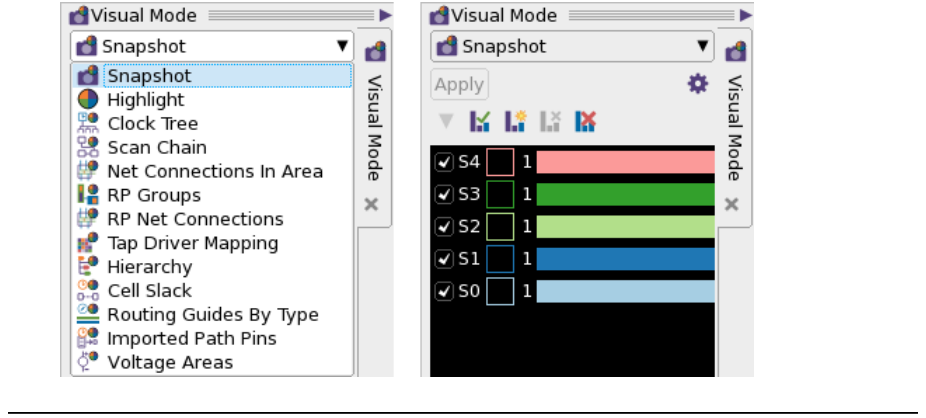
\includegraphics[width=0.92\textwidth]{gui-fig-098.png}
\caption{Visual 模式}
\label{fig:gui-98}
\end{figure}

\section{快照 Visual 模式}
\subsection*{Snapshot Visual Mode}

使用快照 Visual 模式（Snapshot Visual Mode）把一组选中对象收集到一个分档中，并施加高亮颜色。从菜单选择 \textbf{Highlight > Color By > Snapshot}，即可启用快照 Visual 模式。

\begin{figure}[htbp]
\centering
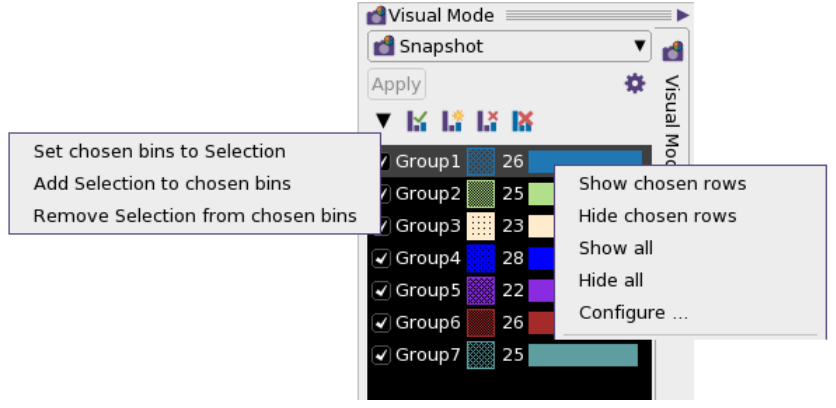
\includegraphics[width=0.92\textwidth]{gui-fig-099.png}
\caption{快照 Visual 模式}
\label{fig:gui-99}
\end{figure}

可以用快照 Visual 模式执行下列操作：
\begin{itemize}
  \item 单击 Copy selection to new bin 按钮，为当前选中的对象着色、创建一个新分档，并把所选对象加入该分档。
  \item 单击 Create a new bin 按钮，创建一个空的新分档。
  \item 单击直方图条以选中该分档，单击面板左侧的向下箭头，并选择 Add selection to chosen bins，即可把选中的对象加入分档。

  使用同一上下文菜单，可以从分档中去掉选中的对象，或用当前选择替换分档中的对象。
  \item 单击某一行以选中它，再单击 Delete chosen row 按钮，即可删除该分档。
  \item 单击 Delete all bins 按钮，从直方图中去掉全部行。
  \item 右键单击直方图行，选择 Set Style，选择新颜色并单击 OK，即可更改高亮颜色。
  \item 右键单击某条直方图条，并在上下文菜单中选择相应项（Move to top、Move up、Move down 或 Move to bottom），即可更改直方图条的顺序或隐藏直方图条。
\end{itemize}

\section{高亮 Visual 模式}
\subsection*{Highlight Visual Mode}

使用高亮 Visual 模式（Highlight Visual Mode）创建直方图，表示按高亮颜色分组后的高亮对象计数。在使用高亮 Visual 模式之前，可以在版图中选中对象并选择 \textbf{Highlight > Selected}，从而高亮这些对象。从菜单选择 \textbf{Highlight > Color By > Highlight}，即可启用高亮 Visual 模式。

\begin{figure}[htbp]
\centering
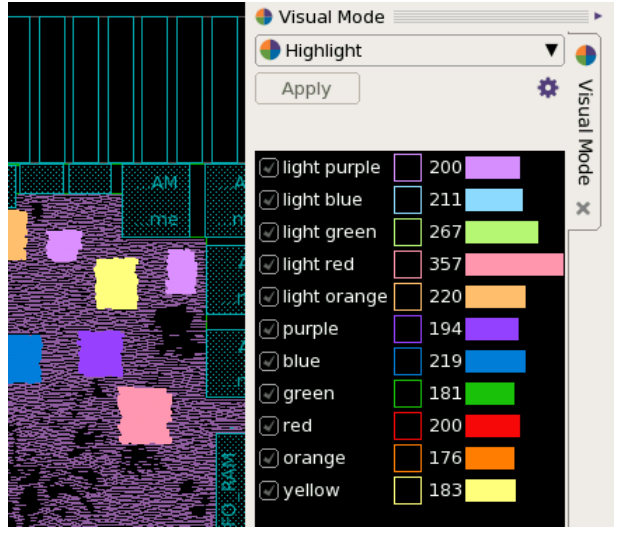
\includegraphics[width=0.92\textwidth]{gui-fig-100.png}
\caption{高亮 Visual 模式}
\label{fig:gui-100}
\end{figure}

在 Highlight Visual Mode 面板中右键单击某条直方图条，可以执行下列操作：
\begin{itemize}
  \item 从上下文菜单选择 Show chosen rows 或 Hide chosen rows，以在版图中显示或隐藏某一直方图行及其对应的高亮颜色。
  \item 从上下文菜单选择 Configure，以配置夸张方案与其他显示选项。
  \item 从上下文菜单选择 Set Style，以更改高亮颜色。
  \item 从上下文菜单选择 Move to top、Move up、Move down 或 Move to bottom，以重排直方图条的顺序。
  \item 选择 Modify Global Selection，并选择用于设置选择、追加选择或从选择中去掉的选项，即可在版图中选中或取消选中已高亮的对象。
\end{itemize}

\section{时钟树 Visual 模式}
\subsection*{Clock Tree Visual Mode}

使用时钟树 Visual 模式（Clock Tree Visual Mode）查看设计中的时钟树，并把相关信息叠加到版图上。

\begin{figure}[htbp]
\centering
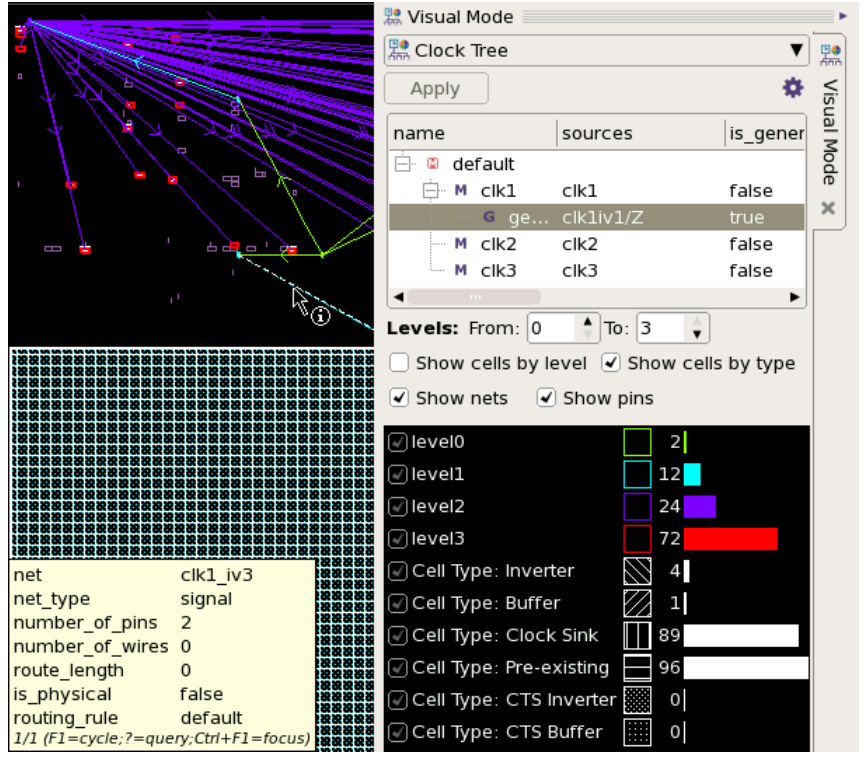
\includegraphics[width=0.92\textwidth]{gui-fig-101.png}
\caption{时钟树 Visual 模式}
\label{fig:gui-101}
\end{figure}

面板显示一张表，列出设计中的时钟源。该表用下列记号显示时钟类型：
\begin{itemize}
  \item M：主时钟（master clock）
  \item G：生成时钟（generated clock）
  \item V：虚拟时钟（virtual clock）
\end{itemize}

面板还显示一张直方图，给出每一级的时钟源、线网与管脚数目，以及每种类型的时钟元件数目。可以用时钟树 Visual 模式执行下列操作：
\begin{itemize}
  \item 单击时钟表中的列标题，按名称、port/pin 或 \cmd{is\_generated} 属性对时钟源排序。
  \item 在面板的 Levels: 部分设置数值，以设定所显示的层次级别范围。
  \item 选择 Show cells by level 选项，按级别显示单元。
  \item 选择 Show cells by type，在版图中加入时钟缓冲器、反相器以及其他单元的单元类型信息。
  \item 选择 Show nets 选项，在版图中显示时钟网飞线（flyline），并把时钟网计数加入直方图。

  选中后，把指针移到时钟网飞线上可显示更多信息。若已做全局布线，工具显示全局布线，而不显示飞线。
  \item 选择 Show pins 选项，显示时钟树中单元的管脚，并把管脚计数加入直方图。
  \item 右键单击直方图行，选择 Set Style，选择新颜色并单击 OK，即可更改高亮颜色。
  \item 在上下文菜单中选择相应项，即可更改直方图条的顺序或隐藏直方图条。
\end{itemize}

\subsection{跟踪时钟树}
\subsubsection*{Tracing Clock Tree}

时钟跟踪器视图提供易于使用的界面，用来跟踪时钟及其相关时钟管脚，一直跟踪到时钟树的漏端管脚。

可以用时钟跟踪器视图：
\begin{itemize}
  \item 优化并调试时钟树综合（clock tree synthesis，CTS）结果；
  \item 查看你可能关心的时钟树漏端。
\end{itemize}

要打开时钟跟踪器视图：
\begin{enumerate}
  \item 选择 \textbf{Window > Clock Tree Analysis Window}。

  把时钟信息载入 CTS 窗口所需的时间，取决于设计是复杂还是简单。复杂设计比简单设计花的时间更长。

  可以过滤时钟与模式，以缩小所显示的信息范围。
  \item 时钟信息载入之后，选择 \textbf{View > Clock Tracer}。

  CTS 窗口按模式组织，显示时钟列表。
\end{enumerate}

要展开时钟树的跟踪，在 CTS 窗口中双击某个时钟或时钟管脚。会出现新的一列，显示该时钟或该时钟管脚所对应的时钟管脚。例如：

单击 Schematic 按钮，可得到时钟层次的图形表示。例如：

使用 Forward 与 Back 按钮，可在时钟层次中导航。

\subsection{检查时钟树重叠}
\subsubsection*{Examining Clock Tree Overlaps}

时钟树重叠分析器视图显示时钟的层次列表或展平列表，以及重叠时钟对的矩阵。重叠矩阵是一个网格，时钟列表中的每个时钟各占一行和一列。

要打开时钟树重叠分析器：
\begin{enumerate}
  \item 选择 \textbf{Window > Clock Tree Analysis Window}。

  把时钟信息载入 CTS 窗口所需的时间，取决于设计是复杂还是简单。复杂设计比简单设计花的时间更长。

  可以过滤时钟与模式，以缩小所显示的信息范围。
  \item 时钟信息载入之后，选择 \textbf{View > Clock Overlap Analyzer}。

  可以过滤时钟与模式，以缩小所显示的信息范围。
\end{enumerate}

在时钟列表中，可展开的层次树表示主时钟与生成时钟之间的时钟层次。可以单击时钟名旁边的展开按钮（加号）来展开该树，从而显示层次中下一级时钟的名称。

重叠矩阵是一个网格，时钟列表中的每个时钟各占一行和一列。矩阵左侧的 Clock 列把列表中的时钟名（包括主时钟与生成时钟）与矩阵中的行、列对应起来。网格中的浅灰色表示这些时钟属于同一时钟域。在时钟列表中选择某个时钟名时，浅蓝色会在矩阵中高亮该时钟所对应的行。背景图案表示哪些时钟处于同一时钟域。

矩阵在网格中显示一个数字，表示该对时钟的重叠点数目。若单击网格中代表一处重叠的方格，工具会在其他视图（例如时钟树原理图或时钟图视图）中用选择色显示该重叠点，选择色默认为白色。

在网格上任意位置右键，可加载上下文相关菜单。菜单中的操作提供更多细节，包括时钟图与时钟属性。从这些细节中可以查看被高亮的重叠点。

\subsection{查看用户定义的偏斜组}
\subsubsection*{Viewing User-Defined Skew Groups}

偏斜组（skew group）使你能够在一个时钟域内平衡不止一组时钟管脚。此外，还可以把集成时钟门控单元（integrated clock-gating cell）的时钟管脚，以及产生时钟的触发器的时钟管脚纳入偏斜组定义，使这些管脚与其他管脚、以及与同一偏斜组定义中的常规漏端一起得到平衡。

使用偏斜组的部分好处：
\begin{itemize}
  \item 可以把与时序关键路径无关的时钟漏端归入一个偏斜组，并放宽该偏斜组的目标偏斜。
  \item 也可以为不同偏斜组分别给出目标早延时（target early delay），从而达到与有用偏斜（useful skew）类似的效果，以改善关键时序路径的裕量（slack）。
\end{itemize}

偏斜组有两种类型：
\begin{itemize}
  \item 默认（Default）：
  \begin{itemize}
    \item 由工具创建；
    \item 每个主时钟定义一个偏斜组，命名为 \cmd{default\_<master\_clock>}；
    \item 这些偏斜组没有与之关联的特定漏端管脚；
    \item 漏端管脚是相关联主时钟的那些管脚。
  \end{itemize}
  \item 用户定义（User-defined）：
  \begin{itemize}
    \item 由用户用 \cmd{create\_clock\_skew\_group} 命令创建；
    \item 每个偏斜组与给定模式相关联；
    \item 每个偏斜组与一份管脚或端口列表相关联。
  \end{itemize}
\end{itemize}

要查看用户定义的时钟偏斜组：
\begin{enumerate}
  \item 选择 \textbf{Window > Clock Tree Analysis Window}。
  \item 选择 \textbf{View > Skew Group Analyzer}。

  时钟树综合窗口同时显示用户定义的时钟偏斜组与默认的时钟偏斜组。

  偏斜组按模式组织。对于用户定义的偏斜组，通往相关联漏端的全部路径都会被高亮。
\end{enumerate}

在时钟树综合窗口中右键单击任意时钟，可以在 Skew Groups 模式与 Clocks 模式之间切换。如下列屏幕截图所示，Skew Groups 模式与 Clocks 模式分别显示与偏斜组、时钟相关的数据。Clocks 模式按时钟显示偏斜组，Skew Groups 模式按偏斜组显示相关时钟。当设计的偏斜组定义很复杂时，这种分类很有帮助。

\begin{figure}[htbp]
\centering
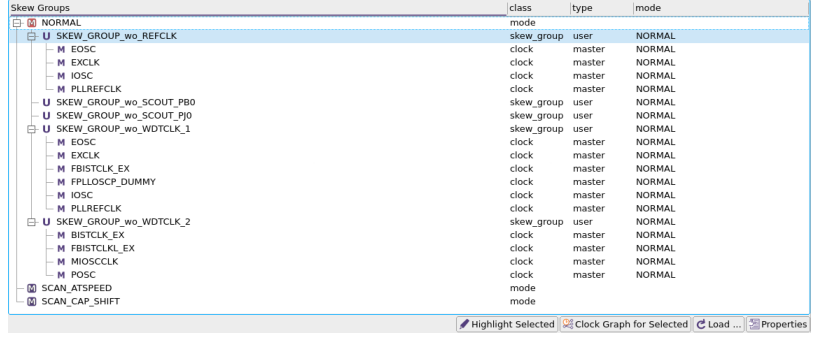
\includegraphics[width=0.92\textwidth]{gui-fig-102.png}
\caption{偏斜组模式}
\label{fig:gui-102}
\end{figure}

\begin{figure}[htbp]
\centering
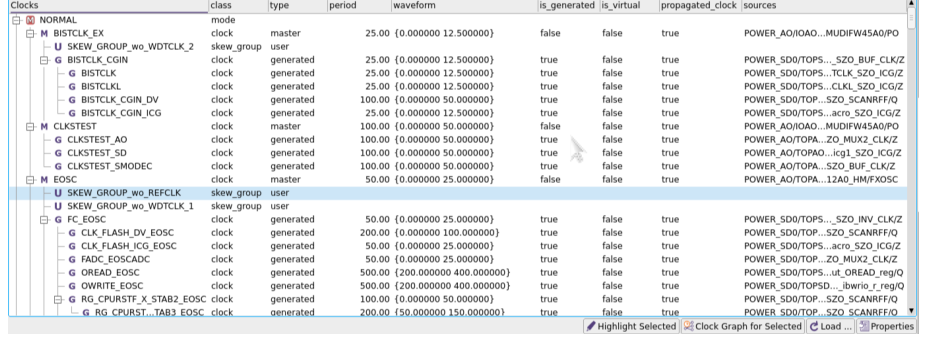
\includegraphics[width=0.92\textwidth]{gui-fig-103.png}
\caption{时钟模式}
\label{fig:gui-103}
\end{figure}

使用 Highlight Selected 菜单，可以在时钟图中高亮所选的时钟或某个偏斜组。例如：

\subsection{查看完整或部分时钟树图}
\subsubsection*{Viewing Full or Partial Clock Tree Graph}

可以用抽象时钟树图（Abstract Clock Tree Graph）查看：
\begin{itemize}
  \item 与该偏斜组的主时钟相关联的全部时钟树；
  \item 只查看与所选用户定义偏斜组相关联的那一部分时钟树。
\end{itemize}

要建立时钟树图：
\begin{enumerate}
  \item 选择 \textbf{Window > Clock Tree Analysis Window}。
  \item 选择 \textbf{View > Skew Group Analyzer}。
  \item 在 CTS 窗口中，右键单击某个偏斜组并选择 Clock Graph。

  打开 Abstract Clock Graph - Levelized 窗口，并显示时钟树。
\end{enumerate}

在该窗口中，也可以查看集成时钟门（integrated clock gate）。

\begin{figure}[htbp]
\centering
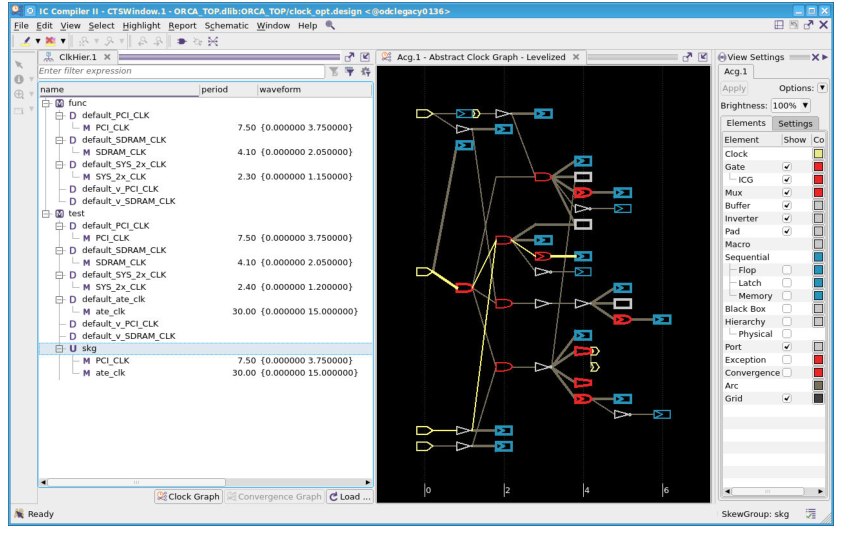
\includegraphics[width=0.92\textwidth]{gui-fig-104.png}
\caption{完整时钟树图}
\label{fig:gui-104}
\end{figure}

\begin{figure}[htbp]
\centering
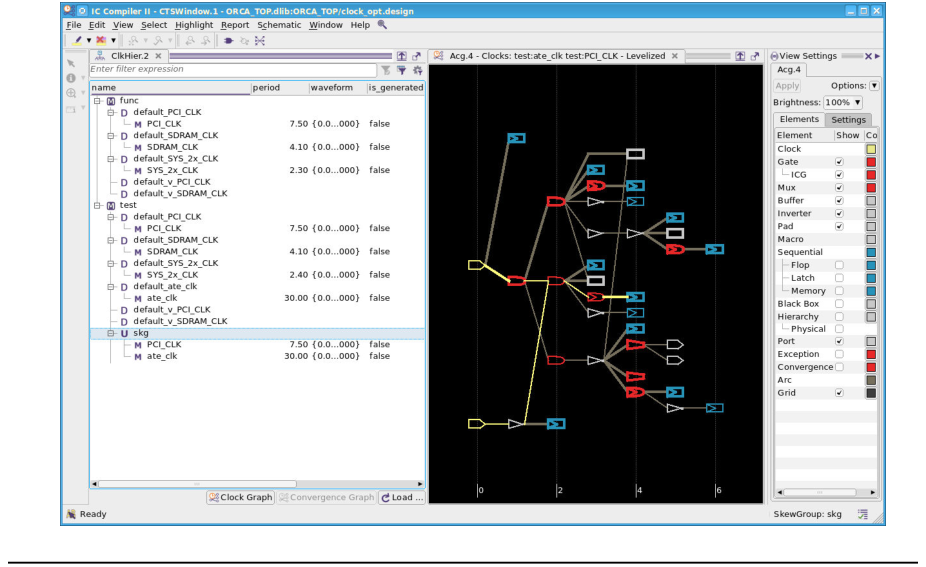
\includegraphics[width=0.92\textwidth]{gui-fig-105.png}
\caption{部分时钟树图}
\label{fig:gui-105}
\end{figure}

\section{扫描链 Visual 模式}
\subsection*{Scan Chain Visual Mode}

使用扫描链 Visual 模式（Scan Chain Visual Mode）显示一条或多条扫描链上扫描输入（scan input）、扫描寄存器（scan register）与扫描输出（scan output）之间的连接。从菜单选择 \textbf{Highlight > Color By > Scan Chain}，即可启用扫描链 Visual 模式。

\begin{figure}[htbp]
\centering
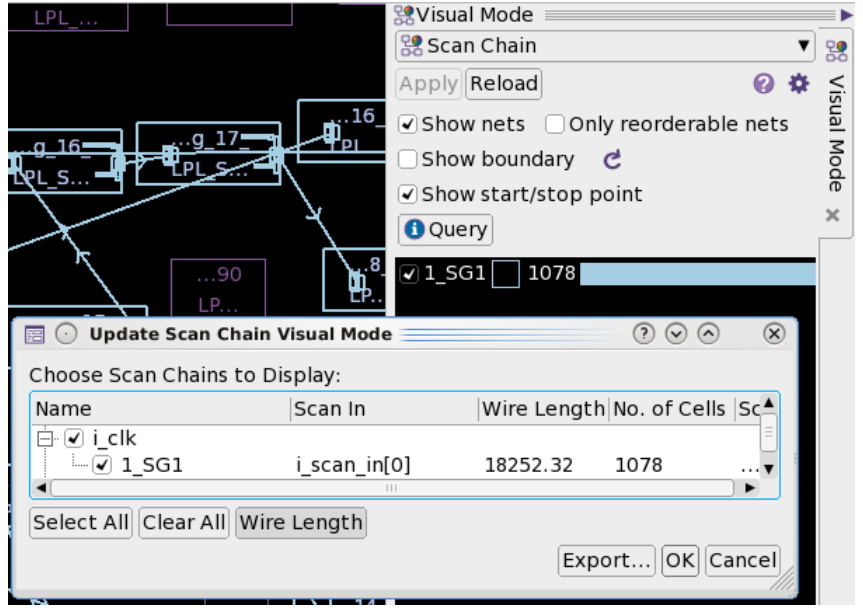
\includegraphics[width=0.92\textwidth]{gui-fig-106.png}
\caption{扫描链 Visual 模式}
\label{fig:gui-106}
\end{figure}

在面板中单击 Reload 之后，可以在 Update Scan Chain Visual Mode 对话框中执行下列操作：
\begin{itemize}
  \item 选中扫描链名称旁边的复选框，并单击 OK 按钮，以在版图窗口中显示所选扫描链。
  \item 单击 Select All 按钮或 Clear All 按钮，对列表中的扫描链执行相应操作。
  \item 单击 Wire Length 按钮，为列表增加一列线长。
  \item 单击某一列并把它拖到新位置，以重排列的顺序。
  \item 把鼠标移到列标题上，单击鼠标右键，并从上下文菜单中选择一项，以配置或排序列表中的列。
\end{itemize}

可以用扫描链 Visual 模式执行下列操作：
\begin{itemize}
  \item 单击 Query 按钮以启动 Query 工具。

  用 Query 工具显示扫描链单元与管脚的更多信息。
  \item 选择 Only reorderable nets 选项，只显示可以重排序的线网。
  \item 选择 Show boundary 选项，显示扫描链的叠加边界。
  \item 选择 Show start/stop point 选项，显示连接到第一条与最后一条扫描链寄存器的端口或管脚连接。
  \item 右键单击直方图行，选择 Set Style，选择新颜色并单击 OK，即可更改高亮颜色。
  \item 在上下文菜单中选择相应项，即可更改直方图条的顺序或隐藏直方图条。
\end{itemize}

\section{区域内线网连接 Visual 模式}
\subsection*{Net Connections in Area Visual Mode}

使用区域内线网连接 Visual 模式（Net Connections in Area Visual Mode）查看与版图中指定区域相交的线网，以帮助在初始布局阶段找出拥塞与布局问题的原因。选择 \textbf{Highlight > Color By > Net Connections in Area}，或单击 Net Connections in Area 按钮，即可启用线网连接 Visual 模式。

\begin{figure}[htbp]
\centering
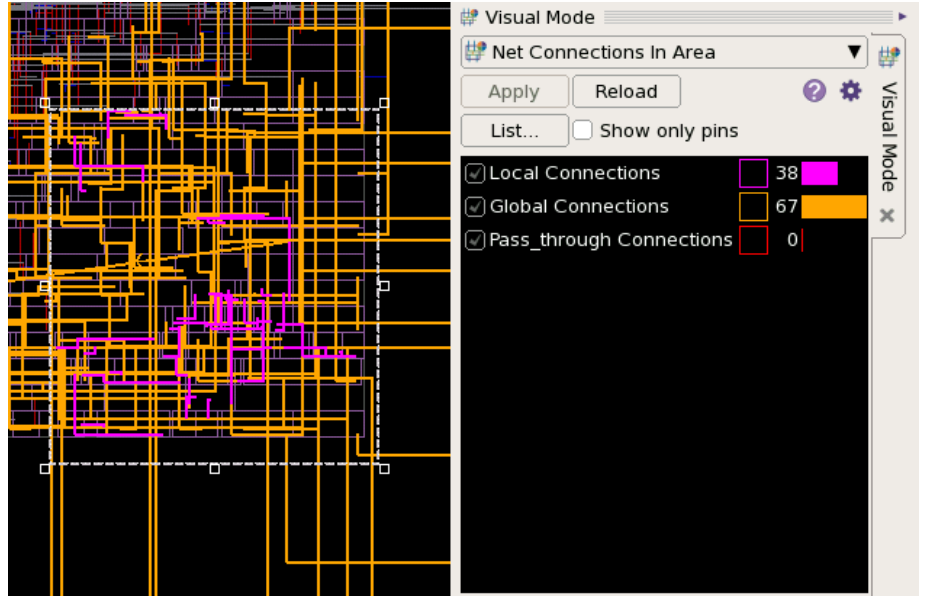
\includegraphics[width=0.92\textwidth]{gui-fig-107.png}
\caption{区域内线网连接}
\label{fig:gui-107}
\end{figure}

工具高亮你所指定区域中的线网，并把它们分成三类：
\begin{itemize}
  \item 局部连接（local connection）：全部管脚与端子都在指定区域之内的线网。
  \item 全局连接（global connection）：至少有一个管脚或端子在指定区域之内，且至少有一个管脚或端子在指定区域之外的线网。
  \item 穿越连接（pass-through connection）：与指定区域相交，但在区域内部没有管脚或端子的线网。
\end{itemize}

要显示指定区域内的线网连接：
\begin{enumerate}
  \item 单击 Reload 按钮，并指定要在其中显示线网的边界框坐标。

  要定义矩形边界，单击区域选择按钮，然后在 Coordinates 框中输入矩形左上角与右下角的 $x$ 与 $y$ 坐标，或在版图视图中拖动指针以形成矩形。
  \item 选择要显示的线网类型（Signal、Clock、Power、Ground、Tie High 或 Tie Low）。
  \item 单击 OK。

  工具显示每一类线网的数目，并按图~\ref{fig:gui-107} 所示在版图窗口中为线网上色。
\end{enumerate}

请注意，图~\ref{fig:gui-107} 显示的是执行全局布线之后的版图。若在执行全局布线之前使用区域内线网连接 Visual 模式，工具显示飞线，而不显示全局布线。

选择 Show only pins，可隐藏工具所高亮的线网，只高亮管脚。修改直方图的更多信息见「配置直方图」。单击 List 按钮，可显示一个对话框，其中包含线网列表，如图~\ref{fig:gui-108} 所示。

\begin{figure}[htbp]
\centering
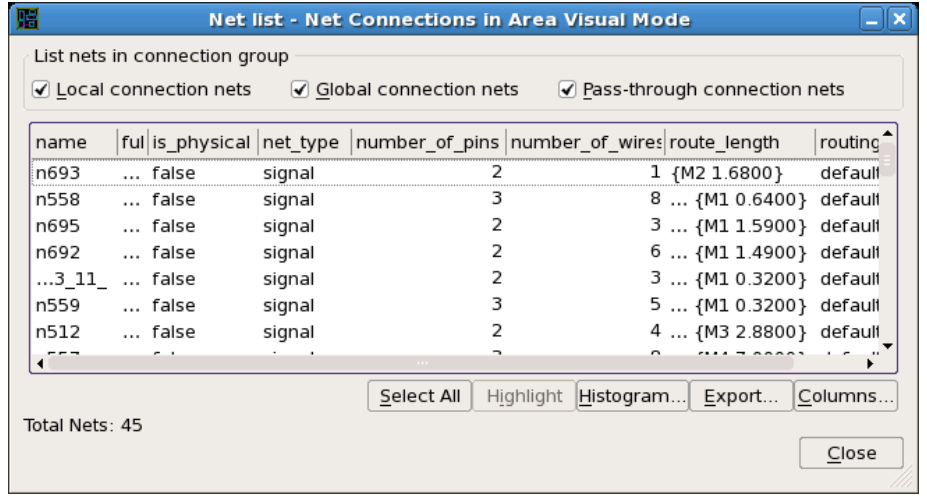
\includegraphics[width=0.92\textwidth]{gui-fig-108.png}
\caption{区域内线网连接列表}
\label{fig:gui-108}
\end{figure}

可以用线网列表对话框执行下列操作：
\begin{itemize}
  \item 单击 Local connection nets、Global connection nets 或 Pass-through connection nets 选项，以切换该线网类型的可见性。
  \item 在线网列表中选择某个线网名，以在版图中高亮该线网。
  \item 单击 Select all 按钮，选择列表中的全部线网。
  \item 单击 Histogram 按钮，配置一个简单直方图，显示区域内的管脚数目或线网数目；在对话框中单击 OK，即可生成直方图，并把它显示在版图窗口的直方图面板中。
  \item 单击 Export 按钮，把表的内容写成逗号分隔值格式的文件。
  \item 单击 Columns 按钮，配置要显示哪些数据列。
\end{itemize}

\section{相对布局（RP）组 Visual 模式}
\subsection*{Relative Placement (RP) Groups Visual Mode}

使用 RP 组 Visual 模式高亮相对布局组。从菜单选择 \textbf{Highlight > Color By > RP Groups}，即可启用 RP 组 Visual 模式。

\begin{figure}[htbp]
\centering
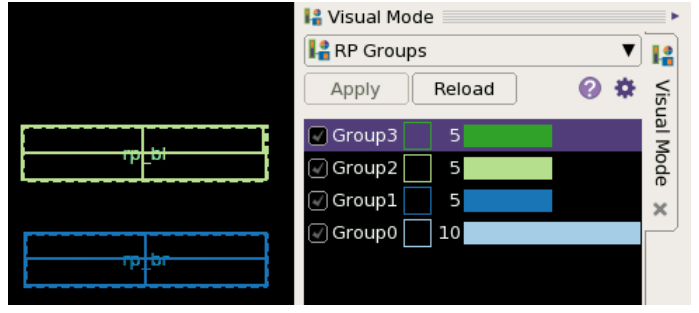
\includegraphics[width=0.92\textwidth]{gui-fig-109.png}
\caption{RP 组 Visual 模式}
\label{fig:gui-109}
\end{figure}

可以用 RP 组 Visual 模式执行下列操作：
\begin{itemize}
  \item 单击 Reload 并单击 OK，高亮设计中的相对布局组。
  \item 选择 Color by RP group，按组名高亮相对布局组。
  \item 选择 Color by RP hierarchical level，按相对布局组在层次中的位置高亮它们。
  \item 选择 Color cell only 选项，只高亮相对布局组中的单元。
  \item 在 Maximum number of colors 框中输入新值，以增加或减少被高亮的组数。可以输入 5 到 20 之间的整数。
  \item 右键单击某条直方图条，选择 Modify Global Selection，并选择用于设置选择、追加选择或从选择中去掉的选项，即可在版图中选中或取消选中相对布局组。
  \item 在上下文菜单中选择相应项，即可更改直方图条的顺序或隐藏直方图条。
\end{itemize}

\section{相对布局（RP）线网连接 Visual 模式}
\subsection*{Relative Placement (RP) Net Connection Visual Mode}

使用 RP 线网连接 Visual 模式高亮连接相对布局组的线网。从菜单选择 \textbf{Highlight > Color By > RP Net Connections}，即可启用 RP Visual 模式。

\begin{figure}[htbp]
\centering
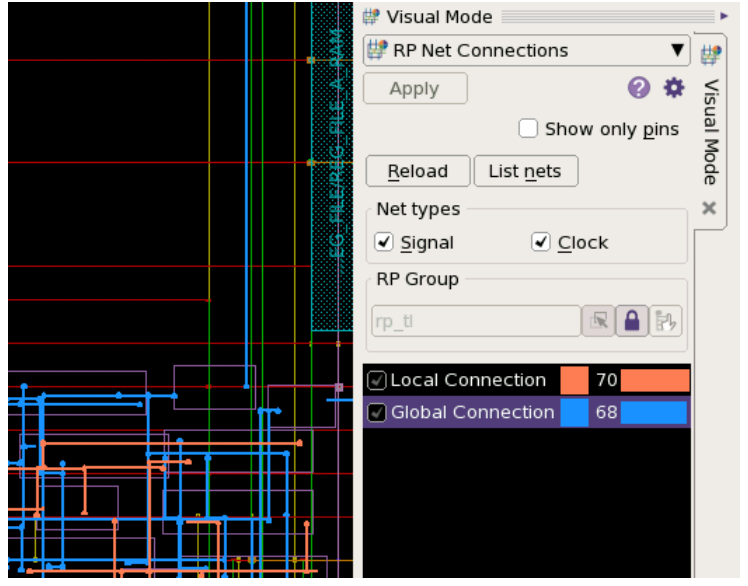
\includegraphics[width=0.92\textwidth]{gui-fig-110.png}
\caption{RP 线网连接 Visual 模式}
\label{fig:gui-110}
\end{figure}

要显示 RP 线网连接：
\begin{enumerate}
  \item 在 RP Group 框中指定一个或多个 RP 组名，或单击 Browse for RP group 按钮并选择一个或多个组。
  \item 选择 Signal 选项以显示信号网，选择 Clock 选项以显示时钟网，或同时选择两项以显示两类线网。
  \item 单击 Reload 按钮，在版图中显示指定 RP 组的 Net Connections。
  \item （可选）单击 List nets 按钮打开对话框，显示指定 RP 组的局部连接与全局连接，如图~\ref{fig:gui-111} 所示。

  用该对话框选择、高亮或导出线网，做法见「区域内线网连接 Visual 模式」。
\end{enumerate}

\begin{figure}[htbp]
\centering
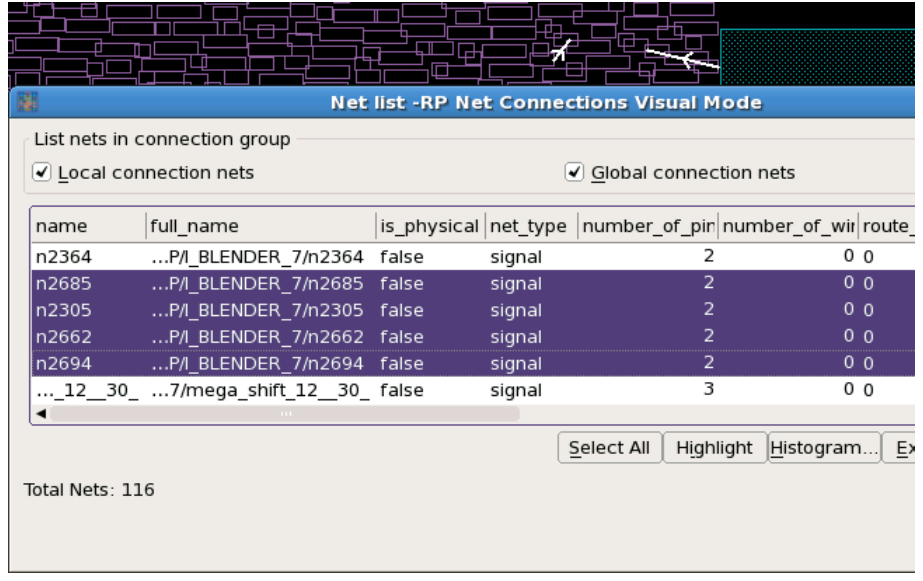
\includegraphics[width=0.92\textwidth]{gui-fig-111.png}
\caption{RP 线网连接列表}
\label{fig:gui-111}
\end{figure}

可以用 RP 线网连接 Visual 模式执行下列操作：
\begin{itemize}
  \item 选择 Show only pins 选项，只高亮连接到 RP 线网连接的管脚。
  \item 选中或取消 Local Connection 或 Global Connection 旁边的复选框，以显示或隐藏 RP 线网连接的飞线。

  局部连接是只连接到同一相对布局组内单元的线网。全局连接至少把相对布局组中的一个单元连接到相对布局组之外的至少一个单元。
  \item 右键单击某条直方图条，选择 Modify Global Selection，并选择用于设置选择、追加选择或从选择中去掉的选项，即可在版图中选中或取消选中相对布局线网连接。
  \item 在上下文菜单中选择相应项，即可更改直方图条的顺序或隐藏直方图条。
\end{itemize}

\section{层次 Visual 模式}
\subsection*{Hierarchy Visual Mode}

使用层次 Visual 模式（Hierarchy Visual Mode）高亮并选择设计中的不同层次级别，或特定的层次单元。从菜单选择 \textbf{Highlight > Color By > Hierarchy}，即可启用层次 Visual 模式。

\begin{figure}[htbp]
\centering
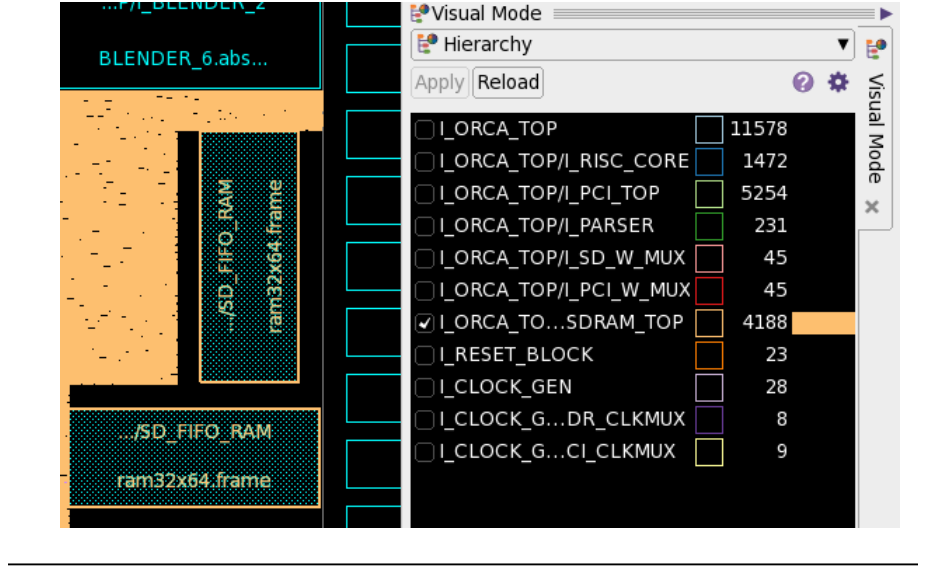
\includegraphics[width=0.92\textwidth]{gui-fig-112.png}
\caption{层次 Visual 模式}
\label{fig:gui-112}
\end{figure}

\section{单元裕量 Visual 模式}
\subsection*{Cell Slack Visual Mode}

使用单元裕量 Visual 模式（Cell Slack Visual Mode）查看设计中的建立（setup）与保持（hold）时序裕量，并把这些信息叠加到版图上。从菜单选择 \textbf{Highlight > Color By > Cell Slack}，即可打开该面板。

\begin{figure}[htbp]
\centering
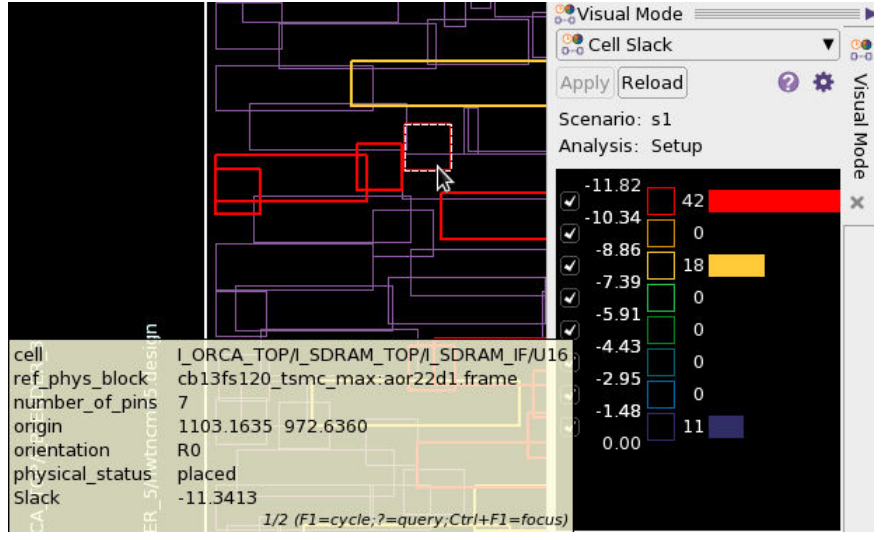
\includegraphics[width=0.92\textwidth]{gui-fig-113.png}
\caption{单元裕量 Visual 模式}
\label{fig:gui-113}
\end{figure}

单击 Reload 按钮，并在对话框中选择选项，即可开始单元裕量分析。设置选项之后，单击 OK 以生成数据。Cell Slack 对话框支持下列操作：
\begin{itemize}
  \item 从框中选择场景（scenario）名称，以指定要分析的场景。
  \item 选择 Setup 或 Hold 选项，以显示建立时间裕量或保持时间裕量信息。
  \item 选择 Number of bins，并选择一个大于零的整数，以指定划分裕量结果所用的分档数目。

  也可以选择 Value range per bin，并指定最小与最大单元裕量值，从而指定每个分档的取值范围。单击 Lower bound strict 或 Upper bound strict 选项，可把指定范围之外的裕量值从直方图中去掉。
  \item 在 Cells 框中输入单元名列表，或选中单元并单击 populate from selection 按钮，以分析特定单元。
  \item 选择 Temperature 或 Gradient 选项，以更改直方图所用的调色板。
\end{itemize}

\section{导入路径管脚 Visual 模式}
\subsection*{Imported Path Pins Visual Mode}

使用导入路径管脚 Visual 模式（Imported Path Pins Visual Mode）在版图中高亮时序路径。从菜单选择 \textbf{Highlight > Color By > Imported Path Pins}，即可启用导入路径管脚 Visual 模式。

\begin{figure}[htbp]
\centering
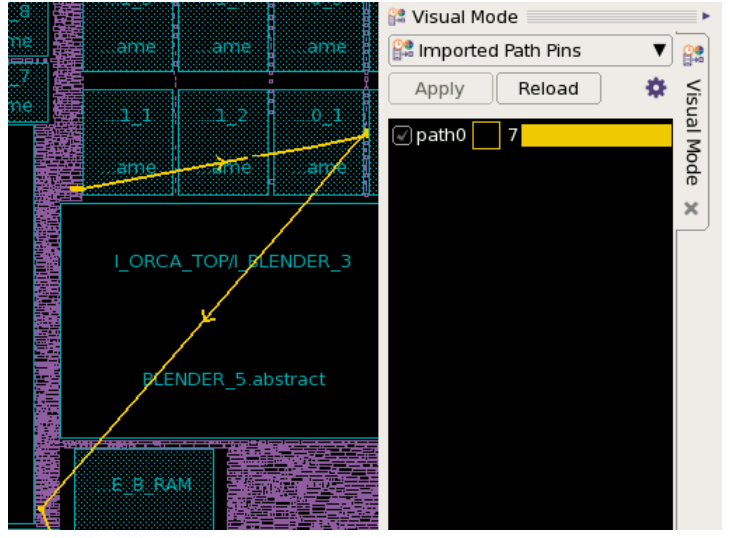
\includegraphics[width=0.92\textwidth]{gui-fig-114.png}
\caption{导入路径管脚 Visual 模式}
\label{fig:gui-114}
\end{figure}

要导入一条时序路径并在版图中高亮该路径：
\begin{enumerate}
  \item 选择 \textbf{Highlight > Color By > Imported Path Pins}，打开导入路径管脚 Visual 模式。
  \item 用 \cmd{update\_timing} 命令更新设计的时序。
\begin{lstlisting}
icc2_shell> update_timing -full
\end{lstlisting}
  \item 用 \cmd{report\_timing} 命令报告一条路径的时序，并把结果保存到文件。
\begin{lstlisting}
icc2_shell> report_timing \
   -from I_RESET_BLOCK/sdram_rst_n_buf_reg \
   -to I_ORCA_TOP/I_SDRAM_TOP/I_SDRAM_IF/DQ_out_1_reg_6_ -nosplit \
   -physical > timing.rpt
\end{lstlisting}
  \item 单击 Reload 按钮。
  \item 选择 Import Path Pins from Timing Report，并单击文件选择按钮。
  \item 选择你在第 3 步写出的 \cmd{timing.rpt} 文件，并单击 OK。

  Imported Path Pins Visual Mode 面板为该路径显示一条直方图条，并给出路径中的管脚数目。工具还会在版图视图中显示该路径的飞线。
  \item 重复第 3 步到第 6 步，以导入并显示更多路径。选择 Clear all buckets before importing new path pins 选项，可在导入新路径之前删除直方图。
\end{enumerate}

除了按第 5 步与第 6 步选择 Import Path Pins 选项并导入文件之外，还可以选择 Import from timing report text，并把时序报告的内容粘贴到文本框中，如图~\ref{fig:gui-115} 所示。

\begin{figure}[htbp]
\centering
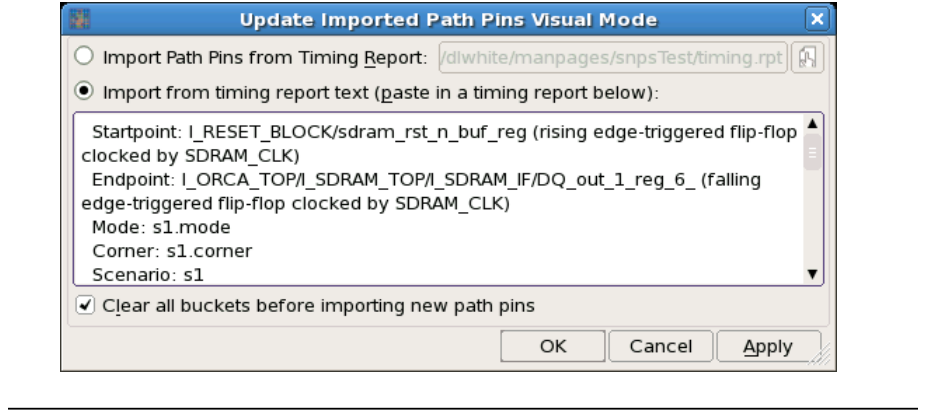
\includegraphics[width=0.92\textwidth]{gui-fig-115.png}
\caption{从时序报告文本导入}
\label{fig:gui-115}
\end{figure}

\section{电压区域 Visual 模式}
\subsection*{Voltage Areas Visual Mode}

使用电压区域 Visual 模式（Voltage Areas Visual Mode）高亮并选择设计中的电源域（power domain）、电平移位器（level shifter）、隔离单元（isolation cell），以及其他与电源域相关的单元。从菜单选择 \textbf{Highlight > Color By > Voltage Areas}，即可启用电压区域 Visual 模式。

\begin{figure}[htbp]
\centering
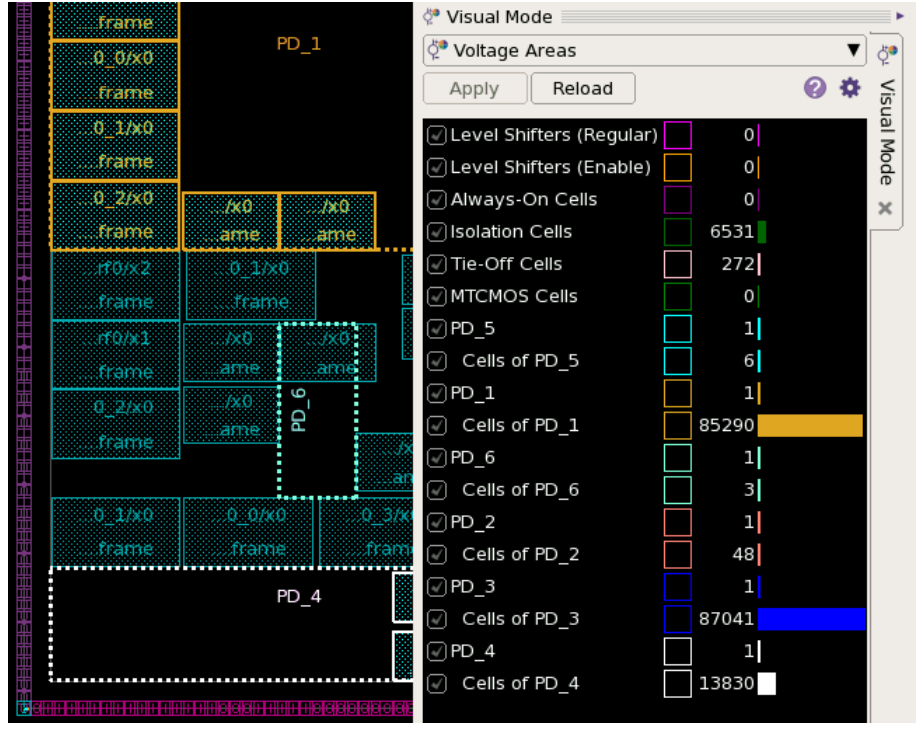
\includegraphics[width=0.92\textwidth]{gui-fig-116.png}
\caption{电压区域 Visual 模式}
\label{fig:gui-116}
\end{figure}

单击 Reload 按钮，以填充 Voltage Areas Visual Mode 面板。右键单击某条直方图条，并从上下文菜单中选择一项，即可更改颜色、在列表中上移或下移该条、在版图中选择相关对象、显示或隐藏该直方图条，以及执行其他操作。
